\documentclass{report}
\usepackage[T1]{fontenc} % Fontes T1
\usepackage[utf8]{inputenc} % Input UTF8
\usepackage[backend=biber, style=ieee]{biblatex} % para usar bibliografia
\usepackage{csquotes}
\usepackage[portuguese]{babel} %Usar língua portuguesa
\usepackage{blindtext} % Gerar texto automaticamente
\usepackage[printonlyused]{acronym}
\usepackage{hyperref} % para autoref
\usepackage{graphicx}
\usepackage{afterpage}
\usepackage{float}

\newcommand\blankpage{%
    \null
    \thispagestyle{empty}%
    \addtocounter{page}{-1}%
    \newpage}


\bibliography{bibliografia}


\begin{document}
%%
% Definições
%
\def\titulo{Projeto Final de LSD }
\def\data{17 de junho de 2021}
\def\autores{Guilherme Craveiro, Rafael Pinto}
\def\autorescontactos{(103574) gjscraveiro@ua.pt, (103379) rafaelpbpinto@ua.pt}
\def\versao{Versão 1}
\def\departamento{Departamento de Eletrónica, Telecomunicações e Informática}
\def\empresa{Universidade de Aveiro}
\def\logotipo{ua.pdf}
%
%%%%%% CAPA %%%%%%
%
\renewcommand{\contentsname}{Índice}
\begin{titlepage}

\begin{center}
%
\vspace*{50mm}
%
{\Huge \titulo}\\ 
%
\vspace{10mm}
%
{\Large \empresa}\\
%
\vspace{10mm}
%
{\LARGE \autores}\\ 
%
\vspace{30mm}
%
\begin{figure}[h]
\center
\includegraphics{\logotipo}
\end{figure}
%
\vspace{30mm}
\end{center}
%
\begin{flushright}
\versao
\end{flushright}
\end{titlepage}

%%  Página de Título %%
\title{%
{\Huge\textbf{\titulo}}\\
{\Large \departamento\\ \empresa}
}
%
\author{%
    \autores \\
    \autorescontactos
}
%
\date{\data}
%
\maketitle

\pagenumbering{roman}

\tableofcontents
% \listoftables     % descomentar se necessário
% \listoffigures    % descomentar se necessário


%%%%%%%%%%%%%%%%%%%%%%%%%%%%%%%
\clearpage
\pagenumbering{arabic}

%%%%%%%%%%%%%%%%%%%%%%%%%%%%%%%%
\chapter{Introdução}
\label{chap.introducao}

\ac{vhdl} é uma linguagem usada para modelar o comportamento e a estrutura de sistemas digitais em, por exemplo, \ac{fpga}. De forma muito resumida, \ac{fpga} é uma matriz de blocos lógicos interligados de modo inteligente que podem ser reprogramados para a aplicação desejada.

Este relatório tem como objetivo explicar o funcionamento da máquina automática de oferta de produtos desenvolvida no nosso projeto. Para que a máquina funcionasse foi necessário a implementação de código em \ac{vhdl} e procedeu-se a vários testes na \ac{fpga} e à análise dos mesmos.

A máquina disponibiliza 3 bebidas diferentes das quais podemos selecionar uma através de \textit{switches}. Após a escolha da bebida o utilizador pode ainda entrar no modo "Modo Escolha tamanho das garrafas", onde pode escolher o tamanho da garrafa, 25cl, 33cl, 50cl ou 10dl. Por defeito está configurado para 33cl. A máquina tem ainda um RESET global que coloca a máquina no estado inicial.

\chapter{Arquitetura}
\label{chap.arquitetura}
\section{Fase 1}
Para a construção da fase 1 deste projeto, tive-se de implementar um temporizador, um divisor da frequência do \textit{clock}, uma máquina de estados e uma estrutura que permitisse escrever mensagens nos \textit{displays} de 7 segmentos, que estão representados na figura \ref{fig:Fase1Estrutura} pelos nomes \textit{TimerFSM}, \textit{ClkDivider}, \textit{Fase1FSM} e \textit{Display}, respetivamente.

A estrutura \textit{ClkDivider} permite dividir a frequência do \textit{clock} de 50 MHz e passar um \textit{clk} de frequência 10 Hz para a estrutura \textit{Display} que irá permitir colocar a palavra "OLA" a piscar à frequência de 10 Hz.

A estrutura \textit{TimerFSM} foi implementada com o intuito de contar os tempos que a palavra "OLA" aparece a piscar nos \textit{displays} de 7 segmentos e o \textit{led} vermelho fica aceso. Quando esta estrutura fica ativada irá fazer uma contagem decrescente com o valor que lhe é passado pela máquina de estados \textit{Fase1FSM}, quando chega a zero envia um sinal para a máquina de estados que significa que o tempo terminou.

A estrutura \textit{Display} é a que vai permitir escrever nos \textit{displays} de 7 segmentos. É ativada pelos \textit{switches} ou, no caso de quando se pretender escrever "OLA", ativada quando recebe um sinal da máquina de estados \textit{Fase1FSM}.

A máquina de estados \textit{Fase1FSM} é a estrutura que nos permite colocar tudo a funcionar de forma síncrona e ordenada.

\begin{figure}[H]
    \centering
    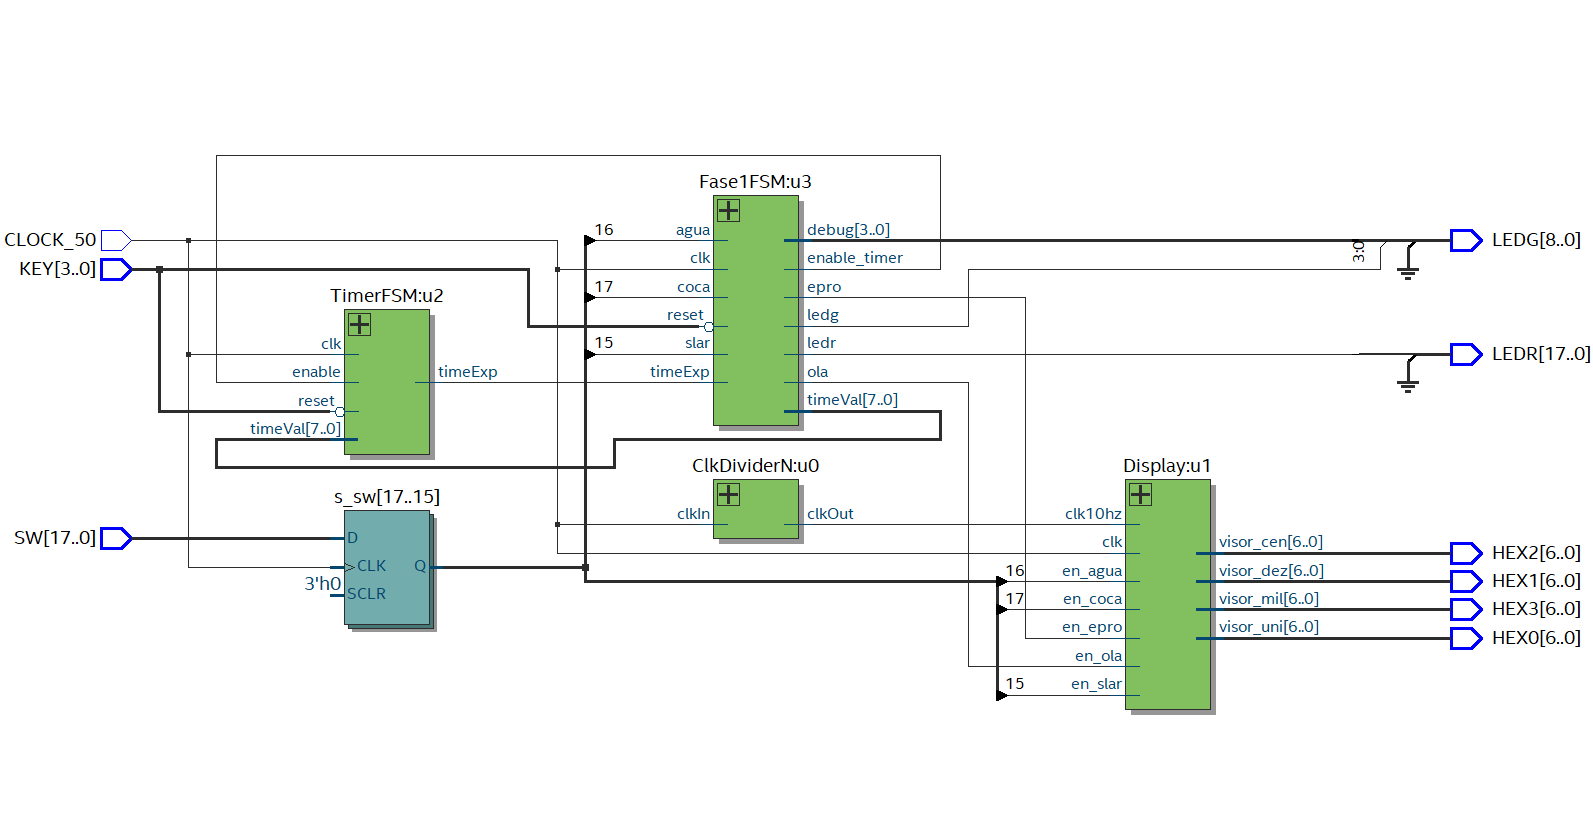
\includegraphics[width = \textwidth]{Fase1Estrutura.png}
    \caption{Arquitetura da Fase 1}
    \label{fig:Fase1Estrutura}
\end{figure} 


\section{Fase 2}

Na implementação da fase 2 acrescentou-se 3 estruturas, que estão representadas na figura \ref{fig:Fase2Estrutura} pelos nomes, \textit{DebounceUnit}, a \textit{Display\textunderscore Tam\textunderscore Garrafa} e a \textit{Sel\textunderscore Tam\textunderscore Garrafa}. Esta fase só é ativada quando o \textit{switch} 0 está ativo no momento em que se escolhe a bebida.

A estrutura \textit{DebounceUnit} gera um pulso de relógio que vai servir para escolher o tamanho da garrafa na estrutura \textit{Sel\textunderscore Tam\textunderscore Garrafa}. Cada vez que é gerado esse sinal a máquina de estados avança para o estado seguinte.

A máquina de estados \textit{Sel\textunderscore Tam\textunderscore Garrafa} é a estrutura que nos permite escolher o tamanho da garrafa.

A estrutura \textit{Display\textunderscore Tam\textunderscore Garrafa} permite visualizar nos \textit{displays} de 7 bits qual o tamanho de garrafa que estamos a escolher.

\begin{figure}[H]
    \centering
    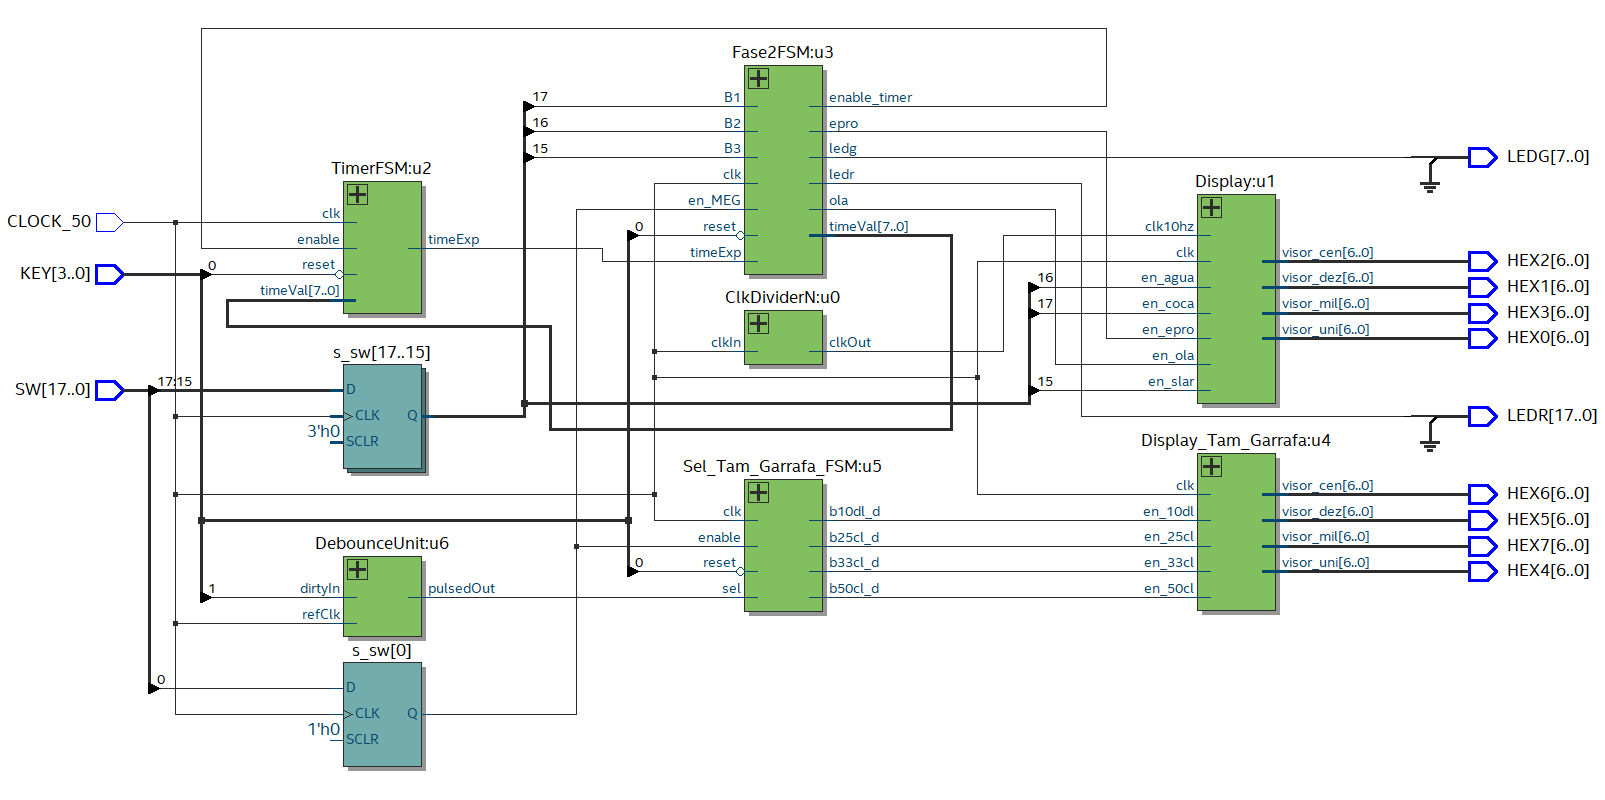
\includegraphics[width = 11cm]{ArquiteturaFase2.png}
    \caption{Arquitetura da Fase 2}
    \label{fig:Fase2Estrutura}
\end{figure}
 


\chapter{Implementação}
\label{chap.implementação}
%%incluindo representação gráfica das máquinas de estado \\%%%finitos
%%implementadas – se aplicável, aspetos de implementação \\\%%mais relevantes e ligação a
%%periféricos do kit%%

\section{Fase 1}

\subsection{Máquina de Estados da Fase 1}

Primeiramente, desenhou-se a máquina de estados que se iria implementar na fase 1 (figura \ref{fig:Fase1FSM}). 

\begin{figure}[H]
    \centering
    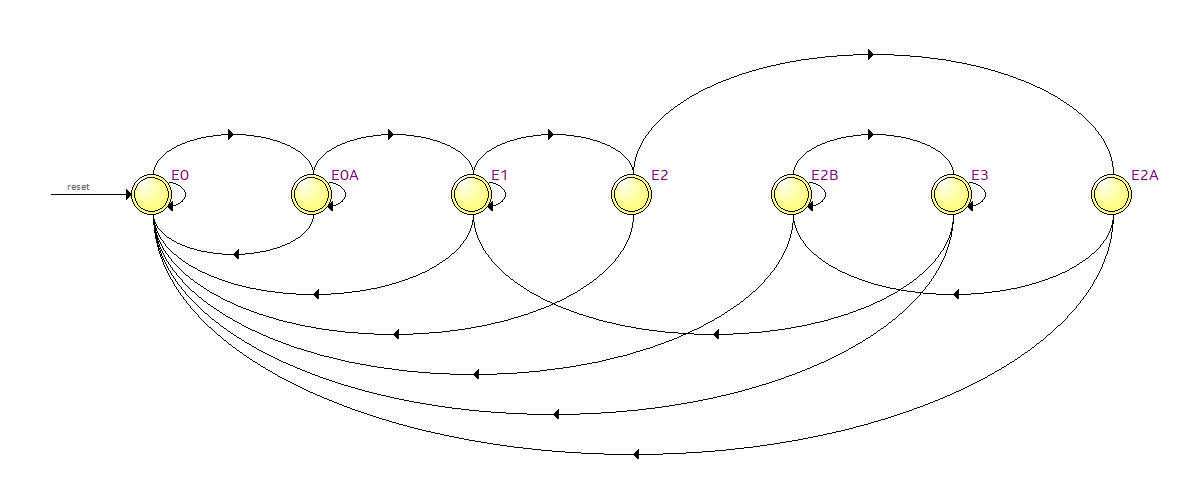
\includegraphics[width = \textwidth]{FSM1.png}
    \caption{Máquina de estados utilizada na Fase 1}
    \label{fig:Fase1FSM}
\end{figure}

A máquina de estados vai permitir que o funcionamento do projeto seja feito de forma síncrona e ordenada. Para a máquina de estados definiu-se um reset que quando ativo põe a máquina de estados no estado inicial e um \textit{clock} que permite que seja criado um processo síncrono. Definiram-se também os \textit{inputs} "coca", "agua" e "slar" que permitem selecionar a bebida pretendida, o \textit{input timeExp} que recebe o sinal do temporizador de que o tempo terminou, os \textit{outputs ola} e \textit{epro} que emitem o sinal ao \textit{Display} para apresentar a mensagem "OLA" e "EPRO", respetivamente, o \textit{output timeVal} que emite o tempo pretendido, o \textit{output enable\textunderscore timer} que emite o sinal para ligar o temporizador e os \textit{outputs ledr e ledg} que emitem o sinal para ligar o \textit{led} vermelho e o \textit{led} verde, respetivamente.

Na arquitetura da máquina de estados definiram-se duas constantes com a duração do piscar da palavra "OLA" e do \textit{ledr} aceso, quatro e seis segundos, respetivamente.
Optou-se por fazer um só processo síncrono. 

No estado E0 os \textit{outputs ola} e \textit{enable\textunderscore timer} são ativos e é passado o tempo do \textit{OLA\textunderscore TIME} para o \textit{output timeVal} que passará como sinal para o temporizador e a máquina avança para o estado E0A que desativa o \textit{enable\textunderscore timer} e quando a contagem do temporizador chega ao fim a máquina avança para o estado E1.

No estado E1 o \textit{output ola} passa a zero e é ativado o \textit{output epro}. Neste estado estamos na fase de escolha de uma bebida, após escolhida a bebida a máquina avança para o estado E2.

No estado E2 estamos na fase de preparação da bebida. Os \textit{outputs ledr} e \textit{enable\textunderscore timer} são ativos e é passado o tempo do \textit{LEDR\textunderscore TIME} para o \textit{output timeVal} que passará como sinal para o temporizador e a máquina avança para o estado E2A que desativa o \textit{enable\textunderscore timer} e avança para o estado E2B que quando a contagem do temporizador chega ao fim avança para o estado E3. Após vários testes da Fase 1 na \ac{fpga} concluímos que o estado E2A era necessário, uma vez que este estado atrasa um ciclo de relógio o que é necessário para que o temporizador não tenha problemas na contagem do tempo.

No estado E3 estamos na fase em que a bebida é disponibilizada. O \textit{output ledg} é ativo e se forem desativados todos os \textit{inputs} das bebidas a máquina irá voltar ao estado E1 em que o utilizador poderá escolher outra bebida.

\begin{figure}[H]
    \centering
    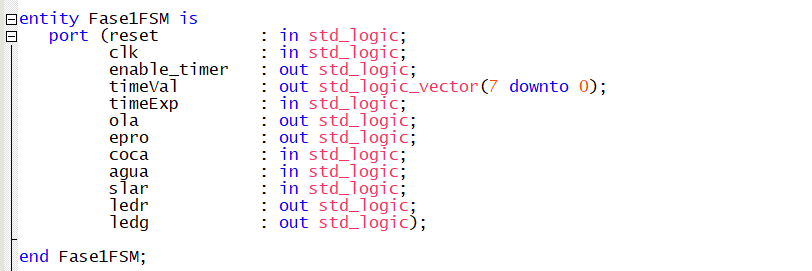
\includegraphics[width = 10cm]{Fase1FSMentity.png}
    \caption{Entidade da máquina de estados}
    \label{fig:entityMáquinadeestados}
\end{figure}

\begin{figure}[H]
    \centering
    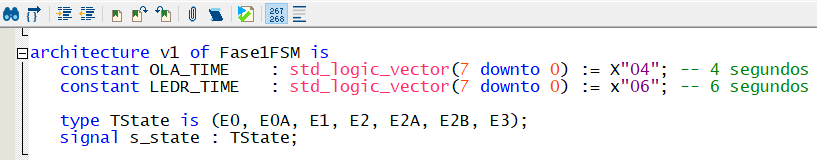
\includegraphics[width = 10cm]{Time.png}
    \caption{Constantes do tempo que o pisca e o led estarão ligados}
    \label{fig:Time}
\end{figure}

\begin{figure}[H]
    \centering
    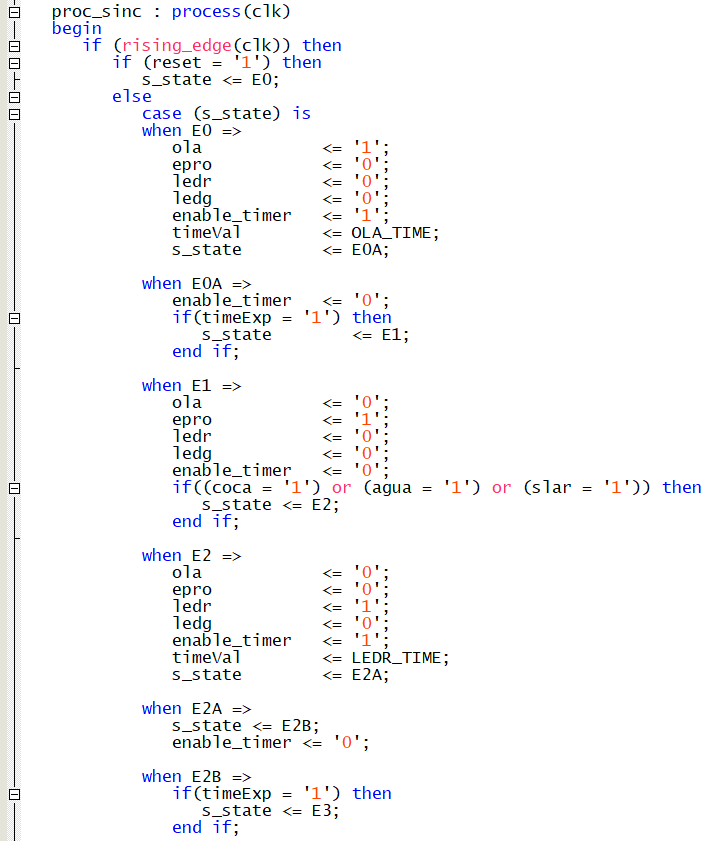
\includegraphics[width = 7cm]{Fase1FSM.png}
   % \caption{Máquina de estados}
    \label{fig:FSM}
\end{figure}

\begin{figure}[H]
    \centering
    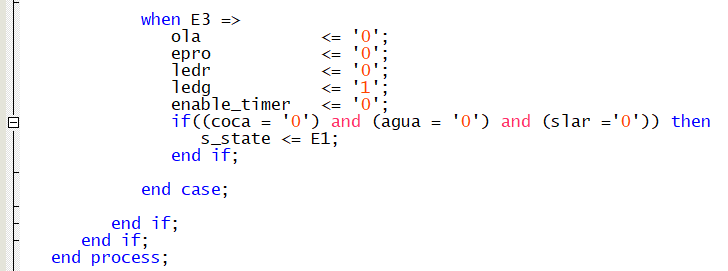
\includegraphics[width = 7cm]{Fase1FSME3.png}
    \caption{Máquina de estados}
    \label{fig:Estado3}
\end{figure}

\newpage

\subsection{\textit{Display}}
De seguida, implementou-se o código necessário para a visualização do texto pretendido nos \textit{displays} de 7 bits. Na entidade do \textit{Display} (figura \ref{fig:Displayentity}) definiu-se um \textit{clock} de 50MHz e outro de 10Hz, o \textit{clock} de 10Hz é usado para criar o efeito da palavra "OLA" a piscar. Definiu-se também \textit{enables} para cada palavra que ia ser escrita e os visores de 7 bits que iriam ser utilizados.

\begin{figure}[H]
    \centering
    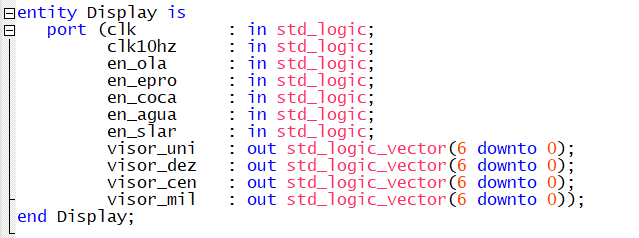
\includegraphics[width = 10cm]{Display1entity.png}
    \caption{Entidade do \textit{Display}}
    \label{fig:Displayentity}
\end{figure}

Na arquitetura do \textit{Display} começou-se por definir constantes para as letras que irão ser usadas nos \textit{displays} (figura \ref{fig:Letras1}), para ser de mais fácil compreensão quando usadas no código implementado. Depois, implementou-se um processo síncrono (figura \ref{fig:Displayprocess}) em que quando o \textit{enable} da palavra é ativo as letras dessa palavra aparecem colocadas no \textit{display} correspondente. Para criar o efeito de piscar da palavra "OLA" usa-se um \textit{clock} de frequência 10Hz (\textit{clk10Hz}). Cada vez que esse \textit{clock} é ativo a palavra é apresentada nos \textit{displays}, quando este está a zero não aparece nada.  

\begin{figure}[H]
    \centering
    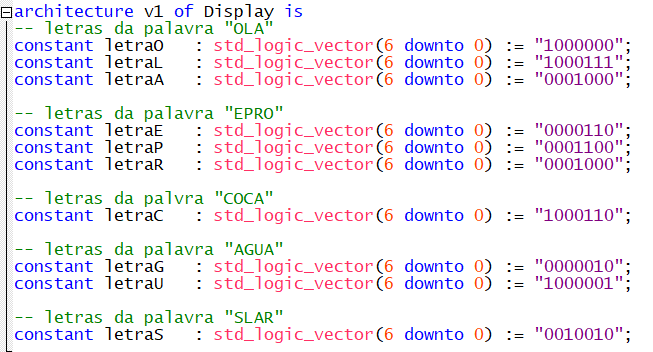
\includegraphics[width = 10cm]{DisplayLetras.png}
    \caption{Constantes para representar as letras nos \textit{displays} de 7 segmentos}
    \label{fig:Letras1}
\end{figure}

\begin{figure}[H]
    \centering
    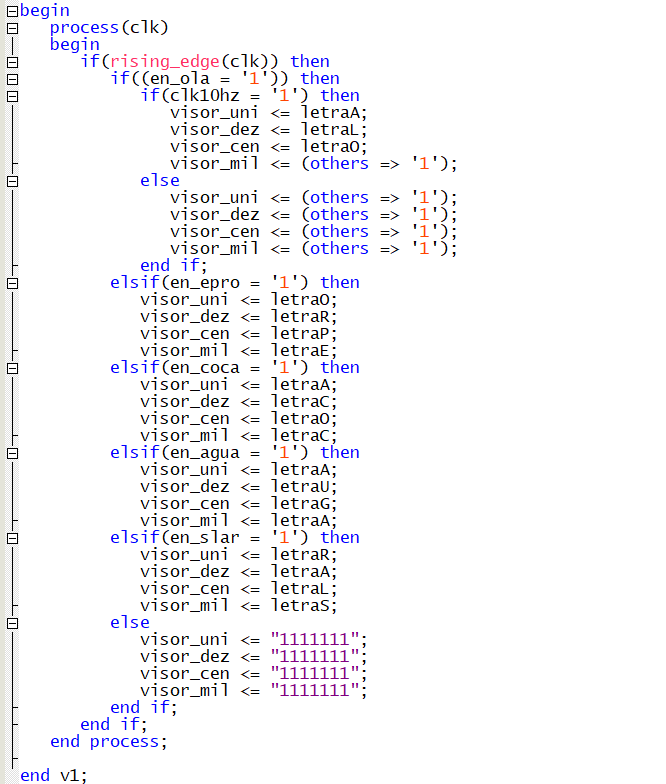
\includegraphics[width = 10cm]{Displayprocess.png}
    \caption{Processo usado para meter as letras nos \textit{displays} corretos}
    \label{fig:Displayprocess}
\end{figure}

\newpage

\subsection{Divisor da frequência \textit{Clock} e Temporizador}

Para que fosse possível a criação de um \textit{clock} de frequência de 10Hz criou-se um código que divide a frequência do \textit{clock} (figura \ref{fig:ClockDivider}). É passado um valor natural à estrutura e esse número vai ser o divisor da frequência do \textit{clock}, neste projeto o valor a ser passado tem de ser cinco milhões.

\begin{figure}[H]
    \centering
    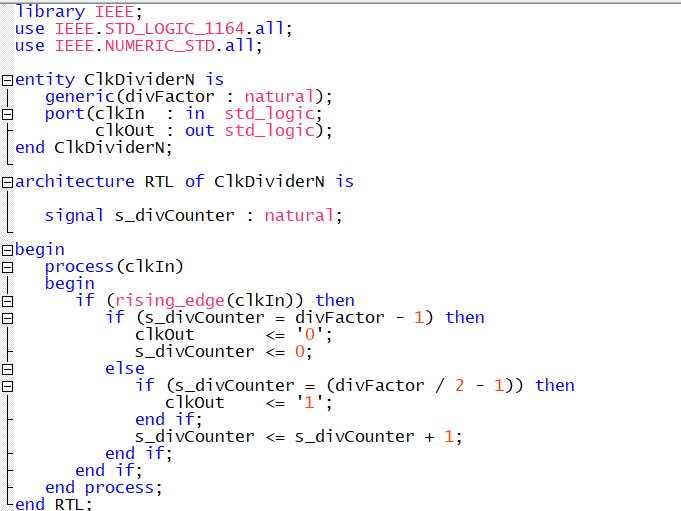
\includegraphics[width = 10cm]{Clockdivider.png}
    \caption{Divisor da frequência do \textit{Clock}}
    \label{fig:ClockDivider}
\end{figure}

Teve-se de implementar, também, um temporizador (figura \ref{fig:Temporizador}) para que seja possível temporizar o tempo do piscar da palavra "OLA" e o tempo que o \textit{led} vermelho deve estar aceso. É passado um valor inteiro à estrutura, esse valor é o tempo em segundos pretendido e é multiplicado pela frequência do \textit{clock} de 50MHz para dar o número de ciclos de relógio que são necessários contar. A cada ciclo de relógio é subtraído um valor ao valor anteriormente calculado, quando esse valor chega a zero é enviado um sinal que significa que o tempo em segundos anteriormente atribuído já passou.

\begin{figure}[H]
    \centering
    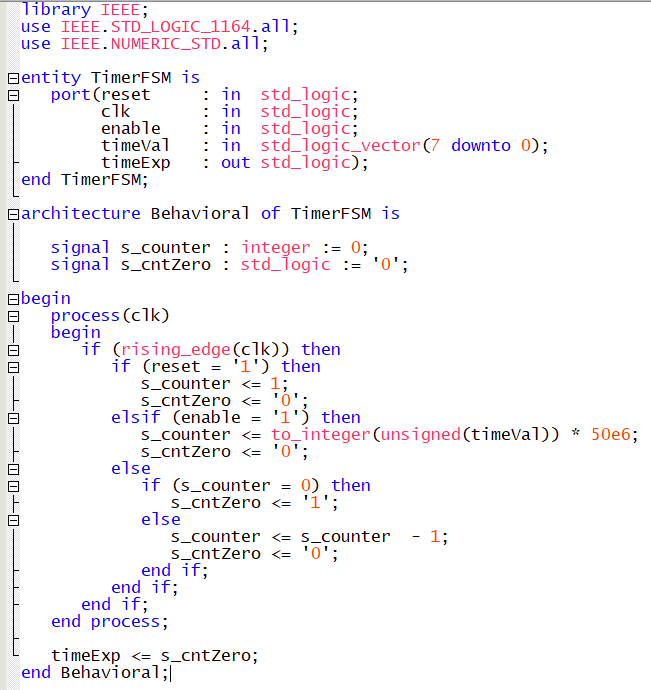
\includegraphics[width = 10cm]{TimerFSM.png}
    \caption{Temporizador}
    \label{fig:Temporizador}
\end{figure}

\newpage

\subsection{\textit{Top-level}}
No \textit{Top-level} é onde se interliga as diferentes estruturas que foram implementadas para que tudo se torne funcional e também é onde são definidos os \textit{switches}, as \textit{keys}, os \textit{displays} de 7 segmentos e os \textit{leds} que serão usados na \ac{fpga}.

Os \textit{enables} de seleção das bebida \textit{coca}, \textit{agua} e \textit{slar}, ligou-se aos \textit{switches} 17, 16 e 15 da \ac{fpga}, respetivamente. Usou-se apenas estes três \textit{switches} na fase 1 do projeto, porém, foi necessário definir todos os \textit{switches} da \ac{fpga}, representado na figura \ref{fig:Switches}, para a máquina funcionar corretamente.

Os visores visor\textunderscore unidades, visor\textunderscore dezenas, visor\textunderscore centenas e visor\textunderscore milhares ligou-se ao HEX0, HEX1, HEX2 e HEX3, respetivamente.

O \textit{ledr} ligou-se ao \textit{LEDR0} e o \textit{ledg} ligou-se ao \textit{LEDG7}, de forma a ficarem próximos um do outro. 

Para o reset global decidiu-se usar uma \textit{key}, neste caso a \textit{KEY0}.

\begin{figure}[H]
    \centering
    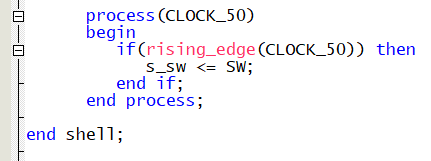
\includegraphics[width = 10cm]{Fase1TopLevelSWs.png}
    \caption{Switches}
    \label{fig:Switches}
\end{figure}

\begin{figure}[H]
    \centering
    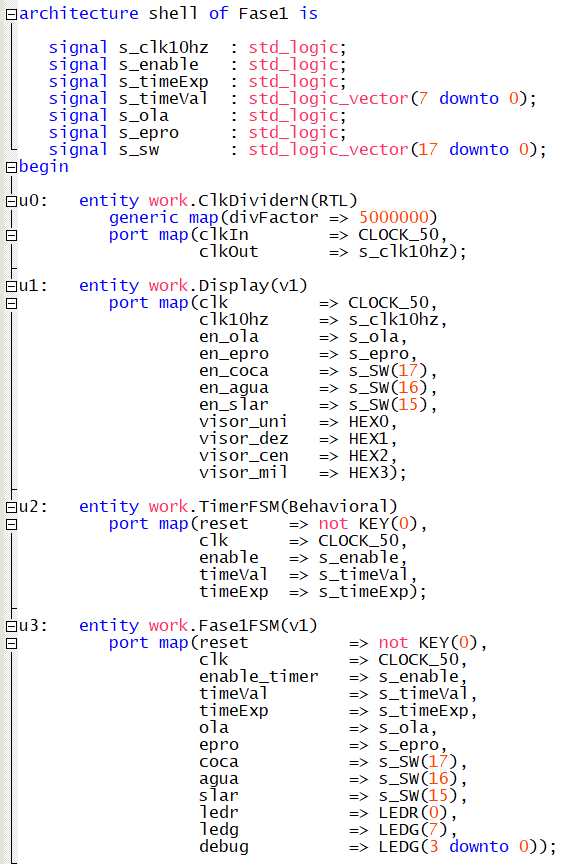
\includegraphics[width = 10cm]{Fase1TopLevelSHELL.png}
    \caption{\textit{Top-level} da Fase 1}
    \label{fig:TLF1}
\end{figure}

\newpage

\section{Fase2}

\subsection{Máquina de estados da Fase 2}
Na fase 2 foi necessário a implementação de mais uma máquina de estados para que fosse possível criar o "modo escolha tamanho das garrafas" (figura \ref{fig:MEGFSM}). Na máquina de estados principal implementou-se mais um estado que só é ativo quando o \textit{enable} do "modo escolha tamanho das garrafas" é ativo (figura \ref{fig:FSMFase2}) e é neste estado que se escolhe o tamanho da bebida. 

A máquina só avança para o novo estado implementado, na figura \ref{fig:FSMFase2} representado por \textit{MEG}, quando o \textit{enable en\textunderscore MEG} estiver ativo. Essa passagem de estado só acontece depois de escolher a bebida, a contagem do tempo do \textit{ledr} do temporizador para e o \textit{ledr} só se desliga quando a máquina sai do estado \textit{MEG}. Quando o \textit{enable} é desativo a máquina avança para o estado E3.

\begin{figure}[H]
    \centering
    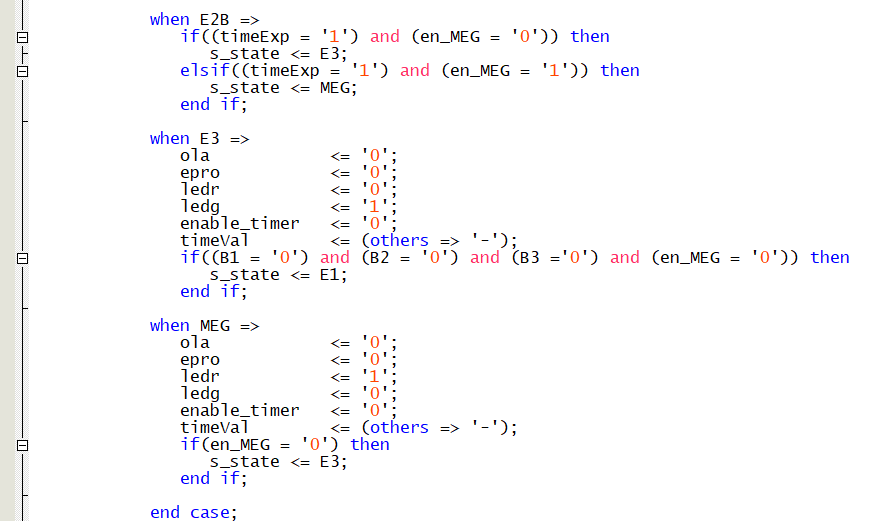
\includegraphics[width = 10cm]{Fase2FSM.png}
    \caption{Novo estado implementado}
    \label{fig:FSMFase2}
\end{figure}

\begin{figure}[H]
    \centering
    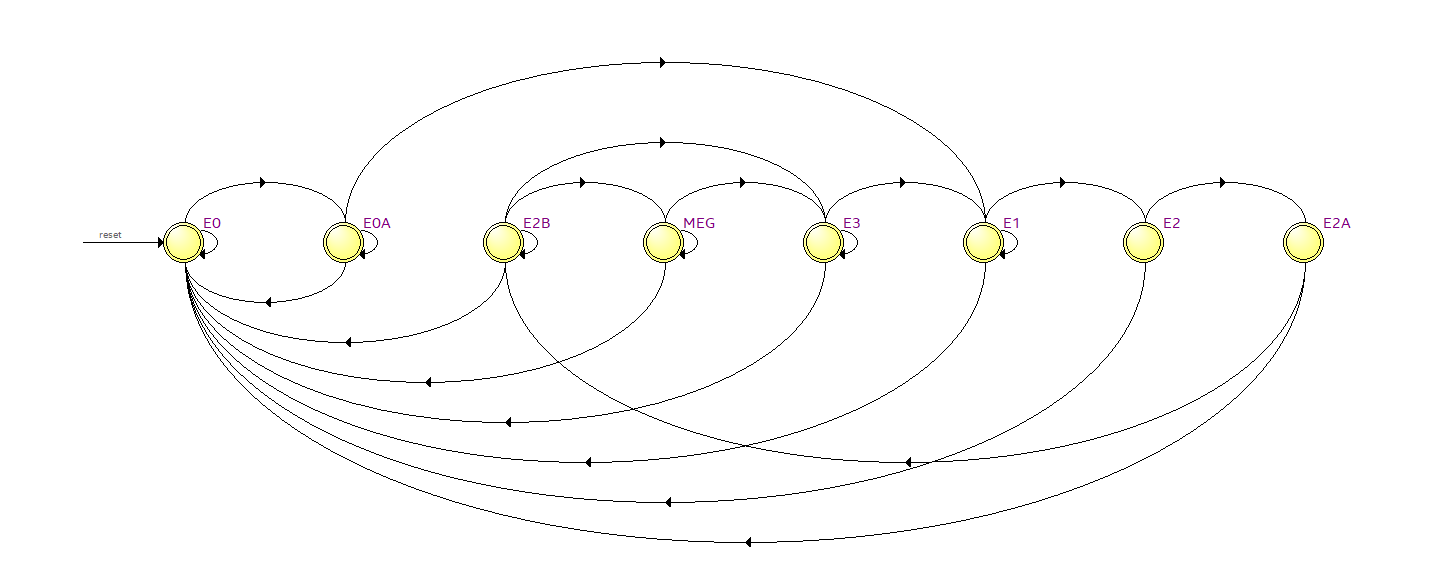
\includegraphics[width = \textwidth]{FSM2.png}
    \caption{Máquina de estados utilizada na Fase 2}
    \label{fig:Fase2FSM}
\end{figure}

Para a máquina de estados implementada para fazer a seleção do tamanho da garrafa (figura \ref{fig:SelFSM}) definiu-se três \textit{inputs}: \textit{sel} que é o sinal enviado pelo \textit{DebounceUnit} implementado posteriormente, \textit{reset} e o \textit{clk} que permite fazer tudo num processo síncrono. E definiu-se quatro \textit{outputs}: \textit{b33cl\textunderscore d, b25cl\textunderscore d, b50cl\textunderscore d e b10dl\textunderscore d} que servem para ativar a quantidade de bebida representada nos \textit{displays}.

Para que a máquina avance de estado é necessário receber um sinal do \textit{DebounceUnit} (\textit{sel}). Por defeito a máquina está configurada para estar no estado 33cl.

Cada vez que há um reset a máquina volta ao estado de 33cl.

\begin{figure}[H]
    \centering
    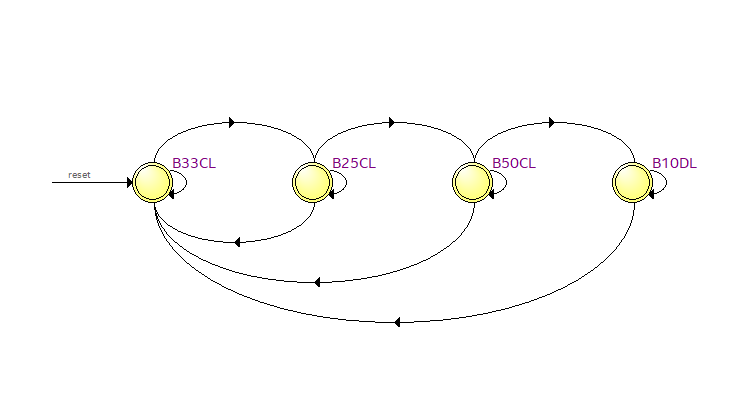
\includegraphics[width = 10cm]{FSMSel.png}
    \caption{Máquina de estados da seleção da garrafa}
    \label{fig:SelFSM}
\end{figure}

\begin{figure}[H]
    \centering
    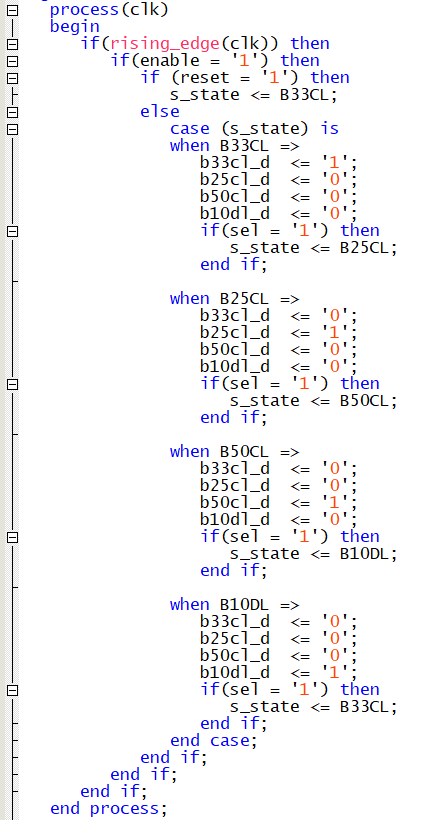
\includegraphics[width = 10cm]{SelFSM.png}
    \caption{Máquina de estados do modo escolha tamanho das garrafas }
    \label{fig:MEGFSM}
\end{figure}

\subsection{\textit{DebounceUnit}}

A única função do \textit{DebounceUnit} é gerar um pulso de relógio cada vez que lhe é enviado algum \textit{input}.

Quando lhe é gerado um \textit{input} é gerado um pulso de relógio que é enviado para a máquina de estados do modo de seleção de bebida e a máquina avança um estado.

\begin{figure}[H]
    \centering
    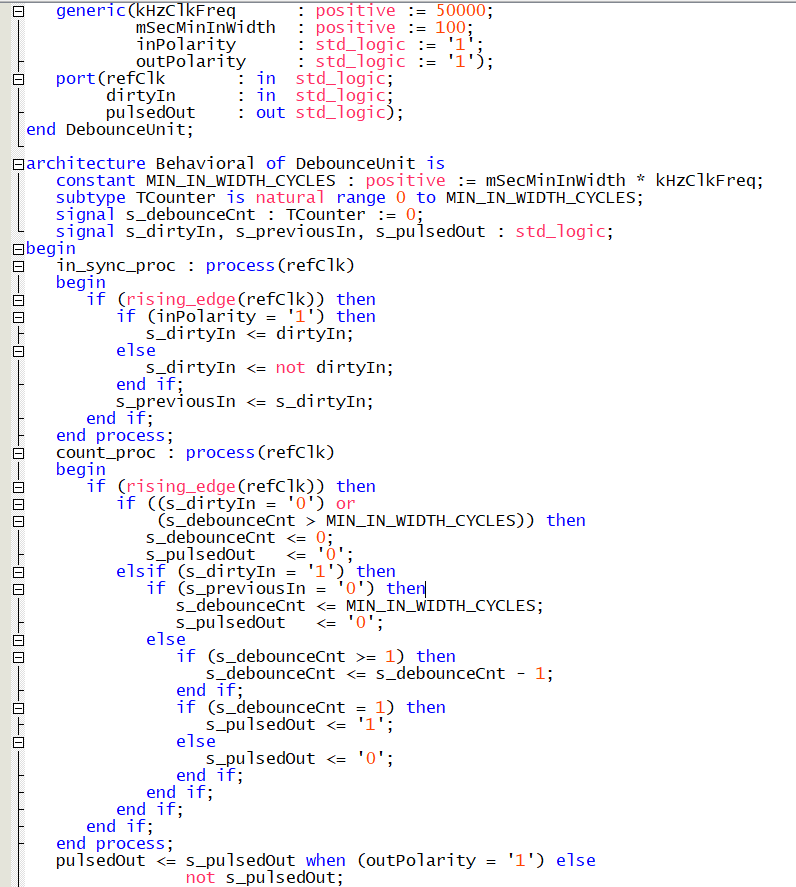
\includegraphics[width = 10cm]{Debounce.png}
    \caption{DebounceUnit }
    \label{fig:Debounce}
\end{figure}

\newpage

\subsection{\textit{Display} do tamanho das garrafas}

A implementação desta estrutura \textit{Display} é idêntica à estrutura implementada na fase 1. Começou-se também por definir constantes para as letras e números a ser usados de forma a que o código escrito posteriormente seja de mais fácil compreensão. Criaram-se \textit{enables} para cada tamanho de garrafa que quando ativo apresenta nos \textit{displays} o tamanho de garrafa correspondente. Quando nenhum está ativo nos \textit{displays} não aparece nada.

\begin{figure}[H]
    \centering
    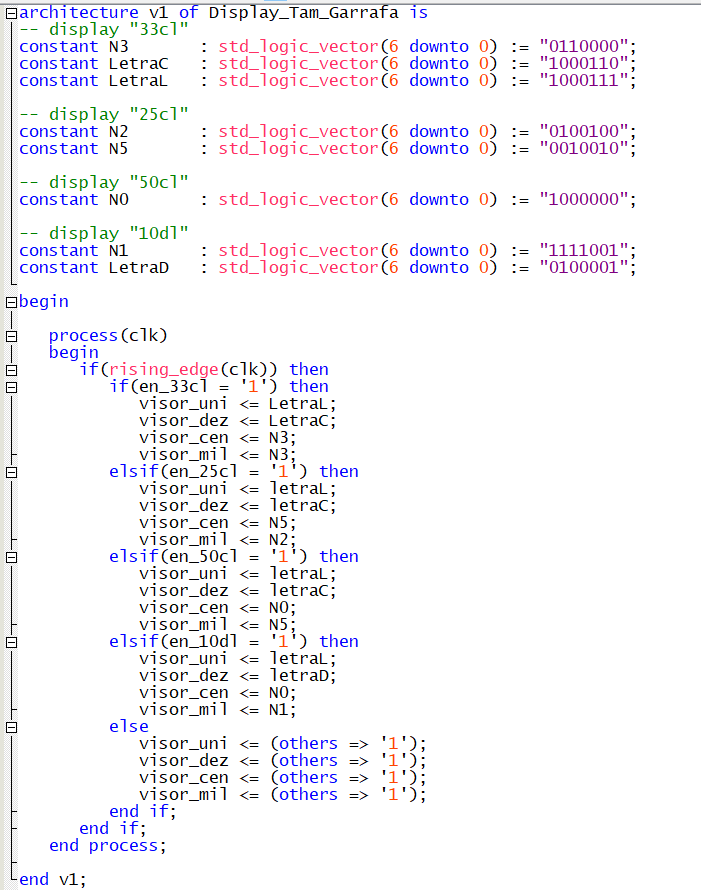
\includegraphics[width = 10cm]{DisplayFase2.png}
    \caption{Display do tamanho das garrafas}
    \label{fig:DispTAmGA}
\end{figure}
\newpage

\subsection{\textit{Top-level}}

No \textit{Top-level} da fase 2 definiu-se sinais do tamanho da garrafa e do pulso de relógio gerado pelo \textit{DebounceUnit} (figura \ref{fig:signals}). Os sinais do tamanho da garrafa servem para ativar os \textit{enables} que ativam a representação do tamanho da bebida que está ser selecionado nos \textit{displays}.

Para gerar o pulso de relógio que permite mudar de estado na máquina de estados da seleção do tamanho da garrafa definiu-se a \textit{KEY1}. Quando se carrega nessa \textit{key} o \textit{DebounceUnit} envia um sinal para a máquina de estados da seleção do tamanho da garrafa e a máquina avança de estado.

O \textit{enable} definido para o "modo Escolha tamanho das garrafas" foi o \textit{switch SW0}.

\begin{figure}[H]
    \centering
    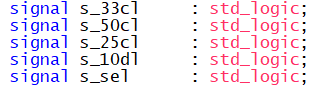
\includegraphics[width = 5cm]{signalsf2.png}
    \caption{Sinais definidos}
    \label{fig:signals}
\end{figure}

\begin{figure}[H]
    \centering
    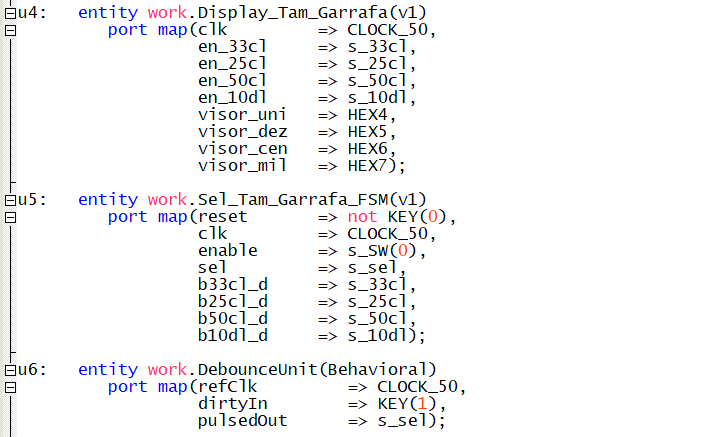
\includegraphics[width = 10cm]{TopLevelF2.png}
    \caption{Top-level Fase 2}
    \label{fig:TL2}
\end{figure}

\chapter{Validação}
\label{chap.validação}
simulação dos principais módulos

\chapter{Manual do utilizador}

Após ligar e programar a \ac{fpga} pressionar a \textit{key} 0 para inicializar a máquina da maneira adequada. Após inicializada a máquina, aparecerá a mensagem "OLA" a piscar durante quatro segundos.

Passados os quatro segundos, nos \textit{displays}, aparecerá a mensagem "EPRO" que significa "Escolha um Produto". Para escolher o produto desejado terá de ativar um dos seguintes \textit{switches}:

\begin{itemize}

\item \textit{Switch} 17: Coca-cola;
\item \textit{Switch} 16: Água;
\item \textit{Switch} 15: Sumo de Laranja.

\end{itemize}

Após a escolha liga-se um \textit{led} vermelho durante seis segundo que significa que a bebida está a ser disponibilizada. Terminando os seis segundos o \textit{led} vermelho desliga-se e liga-se um \textit{led} verde que significa que a bebida já está disponibilizada.

Se o utilizador pretender escolher outra bebida, basta desativar o \textit{switch} que selecionou e aparecerá no \textit{display} a mensagem "EPRO" podendo, assim, selecionar outra bebida.

O utilizador pode ainda entrar no modo "Modo Escolha tamanho das garrafas", onde poderá escolher o tamanho da garrafa, tendo como opções 25cl, 33cl, 50cl ou 10dl. Por defeito a máquina está configurada para disponibilizar garrafas de 33cl. Para entrar neste modo basta, ou antes de disponibilizar a bebida ou enquanto a bebida estiver a ser disponibilizada, ativar o \textit{switch} 0. Para escolher de entre os vários tamanhos de garrafa pressionar a \textit{key} 1. Após selecionar o tamanho da garrafa desative o \textit{switch} 0 e a bebida será disponibilizada na garrafa desejada ligando-se o \textit{led} verde quando estiver pronta. 

Para que a máquina volte ao estado inicial é só pressionar a \textit{key} 0.

\chapter{Conclusões}
\label{chap.conclusao}
Em suma, pode-se afirmar que o projeto cumpre com as especificações e requisitos definidos. Obteve-se uma máquina totalmente funcional, em que é possível escolher a bebida pretendida, bem como o tamanho da garrafa desejado. 

Este projeto permitiu-nos perceber melhor como funcionam os sistemas digitais, principalmente a linguagem \ac{vhdl} que foi usada para modelar o comportamento e a estrutura de tais sistemas. É de salientar que as temáticas abordadas neste projeto são bastante relevantes não só para o nosso percurso académico mas também para uma futura vida profissional.

Sistemas digitais estão presentes em todas as máquinas que nos rodeiam, pelo que o ser humano, mesmo sem se aperceber, se tornou dependente de tais sistemas. Dito isto, achamos que é de extrema importância perceber como os sistemas digitais funcionam e este trabalho ajudou-nos nesse sentido.

\chapter*{Contribuições dos autores}
Este trabalho foi realizado por Guilherme Craveiro (GC) e Rafael Pinto (RP), alunos do primeiro ano do \ac{miect}. Cada um dos autores participou ativamente e de forma conjunta neste trabalho de aprofundamento, permitindo afirmar que tanto o autor GC como o autor RP contribuíram 50\% cada para o aspeto final deste projeto. 

%%%%%%%%%%%%%%%%%%%%%%%%%%%%%%%%%
\chapter*{Acrónimos}
\begin{acronym}
\acro{ua}[UA]{Universidade de Aveiro}
\acro{miect}[MIECT]{Mestrado Integrado em Engenharia de Computadores e Telemática}
\acro{lei}[LEI]{Licenciatura em Engenharia Informática}
\acro{glisc}[GLISC]{Grey Literature International Steering Committee}
\acro{lsd}[LSD]{Laboratórios de Sistemas Digitais}
\acro{vhdl}[VHDL]{VHSIC Hardware Description Language}
\acro{fpga}[FPGA]{Field Programmable Gate Array}
\end{acronym}


%%%%%%%%%%%%%%%%%%%%%%%%%%%%%%%%%
\printbibliography

\end{document}